\documentclass{article}

% Language setting
% Replace `english' with e.g. `spanish' to change the document language
\usepackage[english]{babel}

% Set page size and margins
% Replace `letterpaper' with `a4paper' for UK/EU standard size
\usepackage[letterpaper,top=2cm,bottom=2cm,left=3cm,right=3cm,marginparwidth=1.75cm]{geometry}

\usepackage{listings}

% Useful packages
\usepackage{amsmath}
\usepackage{graphicx}
\usepackage{tikz}
\usepackage[colorlinks=true, allcolors=black]{hyperref}
\usepackage{graphicx}

\usetikzlibrary{positioning,shapes,arrows, calc}

\tikzstyle{stage} = [rectangle, rounded corners, minimum width=2.5cm, minimum height=0.7cm,text centered, draw=black]
\tikzstyle{arrow} = [thick,->,>=stealth]

\title{Senior Project: Winter Quarter Update}
\author{Alex MacLean}

\linespread{1.05}

\begin{document}
\maketitle

\section{Goals}

Over the course of the quarter I've had the opportunity to refine and update my goals based on what I've learned. I'm interested broadly in building an integrated automatic speech recognition system specifically for programming. Existing vocal programming tools work as separate layers that perform basic replacement after speech recognition is complete. These systems can be inaccurate and are geared towards expert users who have learned a large set of specific vocal commands which translate to symbols or hot-keys. I'm working on building a more accurate and new-user-friendly system by integrating static-analysis and knowledge about the language syntax into the audio decoding and by developing a verbal syntax that does more than just directly translate into the surface syntax of the written language.

I'm still pursing my initial goal of building something that can turn ``define a function factorial that takes an int n if n equals zero return one otherwise return n times factorial of n minus one.'' into a corresponding program, But I've revised my understanding of what the challenging parts of this will be and how abstract and flexible I'll be able to make my system.

\section{Progress}

Progress so far has proceeded along two independent tracks: integrating a custom model based on static analysis with speech recognition and implementing a verbal syntax for a programming language. While my initial schedule called for exclusive focus on improving accuracy with a custom language model, after achieving some success in this area I became blocked by the need to define a system to verbally describe programs.

\subsection{A Programming Language Model for Speech Recognition}

To improve accuracy of speech recognition for programming, I spent the first half of this quarter working on integrating a custom language model within an existing speech to text system. Automatic speech recognition systems often work by combining an acoustic model, which assigns probabilities to words based on the audio, with language models, which assign probabilities based on which sequences of words are likely in the language. The probabilities these two models generate are then processed and together produce more accurate transcription then an acoustic model alone. One common type of language model used for speech to text is an $n$-gram model. This model works by recording the probability distribution of tokens after a given $n$ tokens. While a model like this works well for a natural language, in the case of a program, assigning a probability score to a piece of text could incorporate whether the text has syntax errors and additional static analysis.

Unfortunately most existing automatic speech recognition systems do not present a sufficiently abstract API to allow for an entirely custom language model. I spent the early weeks of the quarter unsuccessfully looking for a system that met my needs. CMUSphinx was discarded because it only provided support for custom $n$-gram distributions, not entirely custom models. While it might have been possible to modify the source code to meet my needs, once I managed to get the system running it proved to have extremely poor accuracy. More accurate systems from Google and Intel were also not appealing options because they allowed only for a list of ``privaleged'' words that would be more likely in the transcript. Eventually I found NVIDIA's NeMo, an open-source library for natural language processing \cite{nemo}. Among other things NeMo provides access to some trained acoustic models. These models use an architecture called Connectionist Temporal Classification (CTC) and produce as output a probability matrix where each letter is assigned a probability for each time-step in the input audio file. Unlike older models, which involve multiple steps with segmentation and phonemes, CTC models convert directly between audio and letters \cite{ctc}. While NeMo offers tools for decoding the output of a CTC model with a custom $n$-gram model, after much effort these proved incompatible with a fully custom language model. Instead I take the CTC output matrix and implement my own version of Beam Search \cite{beam}.

To create a programming language model I use existing language servers for static analysis. Language servers are made by the developers of a language so that IDEs (language clients) can implement language specific features like syntax highlighting and auto-completion \cite{lsp}. My language model implements the basic language client protocol to use auto-completion data to score a program. This model is passed as the scoring function to my Beam Search implementation which repeatedly queries the model with possible sequences from the CTC matrix to build a transcription.

\begin{figure}[h]
    \centering
    \vspace{0.5cm}

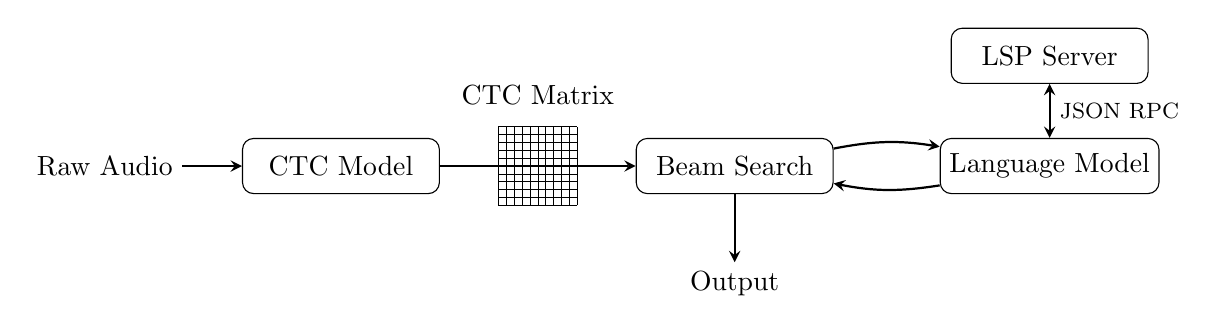
\begin{tikzpicture}[]

\node (aud) [] {Raw Audio};
\node (ctc) [stage, right of=aud, xshift=2cm] {CTC Model};

\node (ctcm) [right of=ctc, xshift=1.5cm, yshift=0.9cm] {CTC Matrix};
\node (beam) [stage, right of=ctc, xshift=4cm] {Beam Search};
\node (lm) [stage, right of=beam, xshift=3cm] {Language Model};
\node (out) [below of=beam, yshift=-0.5cm] {Output};

\node (lsp) [stage, above of=lm, yshift=0.4cm] {LSP Server};


\draw[step=0.1cm,very thin] (5,-0.5001) grid (6.001,0.5);

% \draw [arrow] (cfg) -- (stack) node [pos=0.5,left,font=\footnotesize] {MINI$^{**}_{AST}$};

\draw [arrow] (aud) -- (ctc);
\draw [arrow] (ctc) -- (beam);
\draw [arrow] (beam) -- (out);
\draw [arrow,<->] (lm) -- (lsp) node [pos=0.5,right,font=\footnotesize] {JSON RPC};

%[thick,->,>=stealth]

\draw (lm) edge[arrow,bend left=10] (beam);
\draw (beam) edge[arrow,bend left=10] (lm);

\end{tikzpicture}
\end{figure}

During the first half of the quarter I was able to get the minimum viable implementation of this system running. I used an existing Python language server \cite{pylsp} and NeMo's QuartzNet CTC model \cite{qua} while implementing my own version of Beam Search and a simple language model using my implementation of a LSP language client. While serious testing and fine tuning were not possible due to the limitation that the system performed no inverse-normalization so it could not represent any code containing non alphabetic characters some promising results were still found. To test the system I recorded myself reading some import statements in python and compared the standard greedy CTC decoding with the output of Beam Search using the programming language model.

\begin{table}[h]
    \centering

\resizebox{\textwidth}{!}{%
\begin{tabular}{ |l|l|l| }
 \hline
 Expected Output & Greedy Decoding & LSP-Based LM Re-scoring \\
 \hline
 \texttt{from json import dumps} & \texttt{from jason import dumps} & \texttt{from json import dumps} \\
 \texttt{from math import trunc} & \texttt{from math import trunk} & \texttt{from math import trunc} \\
 \texttt{from threading import enumerate} & \texttt{from threading import enumerate} & \texttt{from threading import enumerate} \\
 \texttt{from torch import cuda} & \texttt{from torch import kuta} & \texttt{from torch import cuda} \\
 \texttt{from itertools import pairwise} & \texttt{from iter tools import peirwise} & \texttt{from itertools import peirwise} \\
 \hline
\end{tabular}}
\end{table}

As seen in the table above, the LSP based language model showed some improvement over the standard decoding in certain import statements. While the improvements are modest, one exciting feature of this approach is that it is totally abstracted away from the programming language. Ideally, any language server could be substituted into the system with only a small amount of effort. While the system still needs some tweaks and further work to improve performance, I was unable to test it more fully until I updated the system to process non-alphabet syntax.

\subsection{Inverse-Normalization for a Verbal Syntax}

During the second half of the quarter I turned my attention to designing a system for verbally specifying Python. Standard speech recognition systems already perform a surprising amount of post-processing on the model output in a process called inverse-normalization. Typically in speech recognition, inverse-normalization is responsible for task such as turning ``twenty twenty two'' into ``2022'' and ``mister'' into ``Mr.''. One popular approach to perform this task is modeled of Google Kestrel, which uses 2 layers of finite-state transducers to transform the text \cite{kes}. The first layer parses the text and identifies phrases which can be normalized and the second layer verbalizes the parsed text \cite{kes}.

For my inverse-normalization layer I chose to mirror this system using a weighted finite-state transducer for the parsing layer and Python's \texttt{tokenize} module for verbalization. While a finite-state machine is not powerful enough to perfectly represent the recursive grammar of a programming language such as Python, by relaxing the grammar it will still be possible to build a machine that accepts all valid programs, in addition to many invalid programs. Unlike standard inverse-normalization, I implement a more state-ful machine which represents being inside of strings or comments with a different set of states, and parses these areas differently. To start I implemented the most basic system possible, where each symbol has a corresponding word which must be spoken. Even this language presented some challenges such as determining when to join multiple words together into a single identifier. I implemented the finite-state transducer using Pynini, a Python library that allows for manipulation of state-machines with operations such as concatenation, union, and closure \cite{pynini}. While this portion of the project still requires significant work next quarter, my inverse-normalize currently supports--if somewhat gracelessly--a specification for a significant subset of Python programs. For example the tokens ``def add bar numbers open paren x comma y comma z close paren colon then return x plus y plus z'' are successfully transformed into the following code:

\begin{lstlisting}
def add_numbers (x ,y ,z ):
	return x +y +z
\end{lstlisting}

In addition I implement a short-hand for defining functions so the same code can be defined by saying ``define add bar numbers of x comma y comma z then ...''. While the system has some serious rough edges around numbers, and inverse-normalization within strings, and many more short-hands should be available for other syntactic forms, I've figured out the basics of the system this quarter and I'm confident next quarter I'll be able to significantly improve it.

\section{Next Quarter}

Next quarter I hope to integrate the inverse-normalization into the automatic speech recognition, improve the verbal syntax supported by inverse normalization, and figure out a more abstract way of specifying the transducer than writing the code that generates the state machine.

\subsection{Revised Schedule}
\begin{enumerate}
    \item Improve the inverse-normalization so that all valid programs are possible to specify, and add more short-hand forms so a user will need to specify fewer symbols.
    \item Integrate the inverse-normalization into the speech recognition, possibly updating Beam Search to only query the language model with complete tokens.
    \item Improve performance and update the system so it works with live input as opposed to transcribing audio files.
    \item Investigate training some portion of the model with a Python corpus mined from GitHub. This could be adding an $n$-gram model to the LM somehow or using speech-to-text to retrain the CTC model.
    \item Cleanup, document, and publish the system so that another person could run it.
\end{enumerate}

\bibliographystyle{plain}
\bibliography{quarter1}

\end{document}